
\section{dbHound: System Design}
\label{sec:system_design}

The dBHound app is designed to simulate a layer between the raw audio stream and voice-enabled mobile applications.
 The applications only receive the obfuscated audio stream for providing their voice-enabled features.
 Any application that requires access to raw audio needs to request for permission from the user every time (Figure \ref{fig:proposed_voice_command_arch}).


The dbHound system is composed of an Android application to interface with the user and collect audio data, and a backend server that obfuscates the audio based on the settings and returns the classification result.
 The app communicates with the backend server using a REST API.
 The app does not access any personal information and all the REST API calls are completely anonymous.
 The only personal information collected is what the user provides when volunteering training data for the dbHound classification system.


Figure \ref{fig:dbhound_submit} shows the screenshot of the \texttt{dbHound Keyphrase} \footnote{The app can be found on the Google Play Store at \url{https://play.google.com/store/apps/details?id=edu.wisc.cs.dbhound}} Android application for users to volunteer training data.
 Figure \ref{fig:dbhound_test} shows the screenshots of the db \texttt{dbHound Keyphrase} application for users to test the keyphrase recognition.
 If the "Classify and Incrementally Train" option is enabled, the trained models are "fine-tuned" based on the user audio and label specified.

\begin{figure}[!th]
\centering
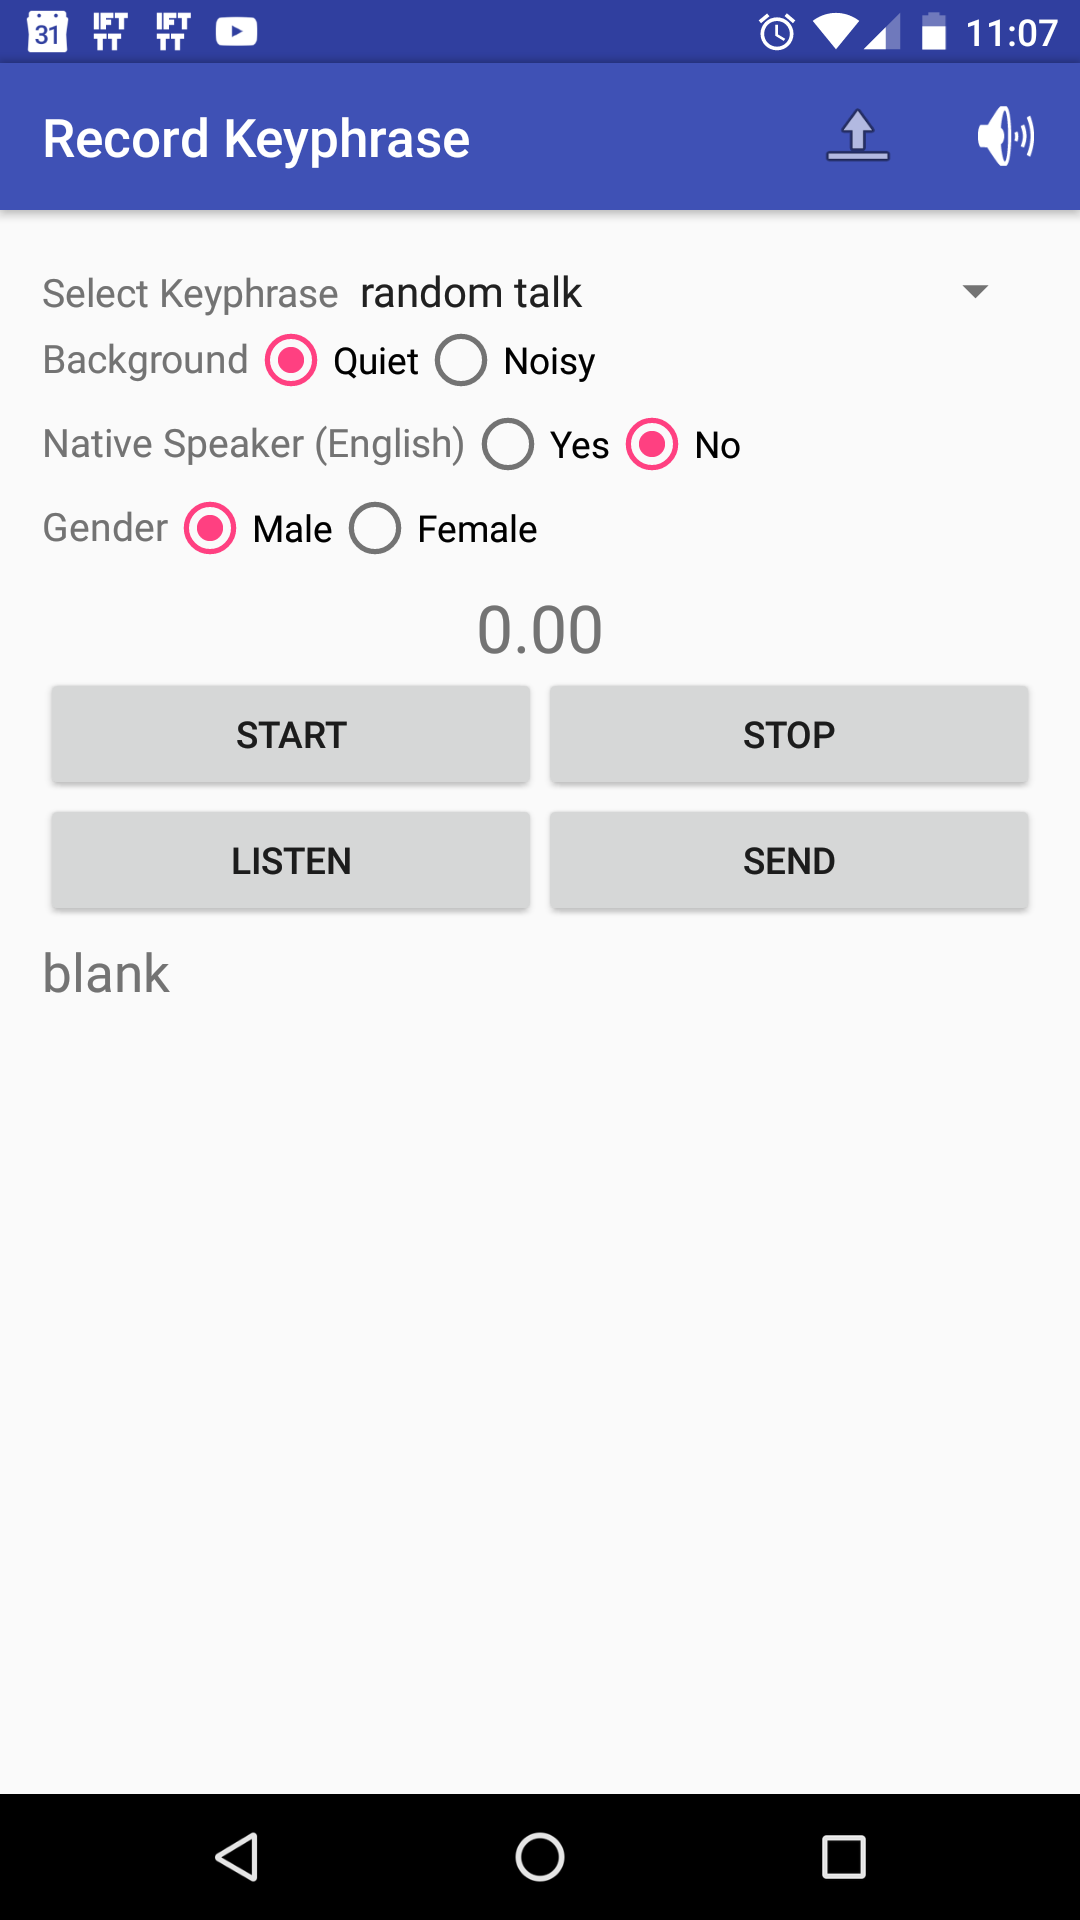
\includegraphics[width=0.25\textwidth]{sound/app_submit.png}
\caption{\texttt{dbHound Keyphrase} Android app screenshot for submitting training data}
\label{fig:dbhound_submit}
\end{figure}

\begin{figure}[!th]
\centering
\begin{subfigure}{0.5\textwidth}
\centering
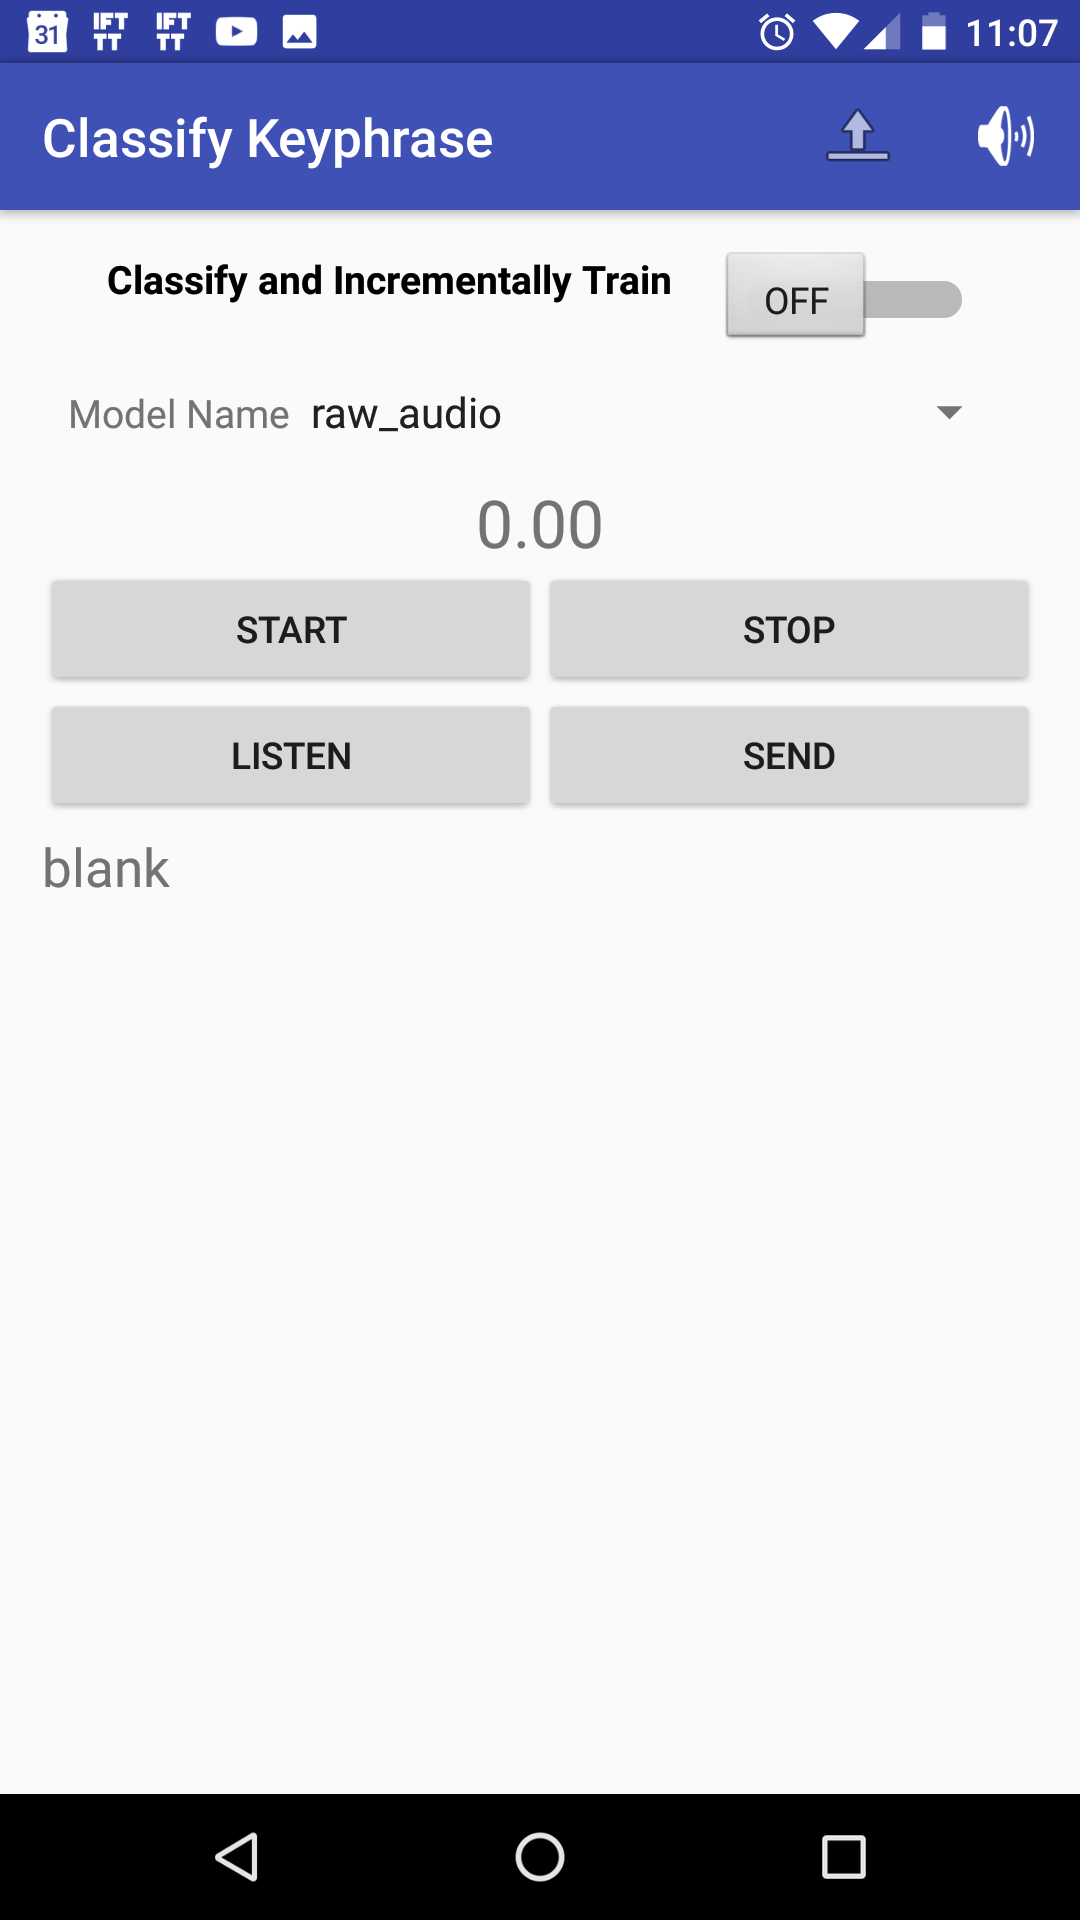
\includegraphics[width=0.5\textwidth]{sound/app_classify.png}
\caption{Only Classify}
\end{subfigure}%
\begin{subfigure}{0.5\textwidth}
\centering
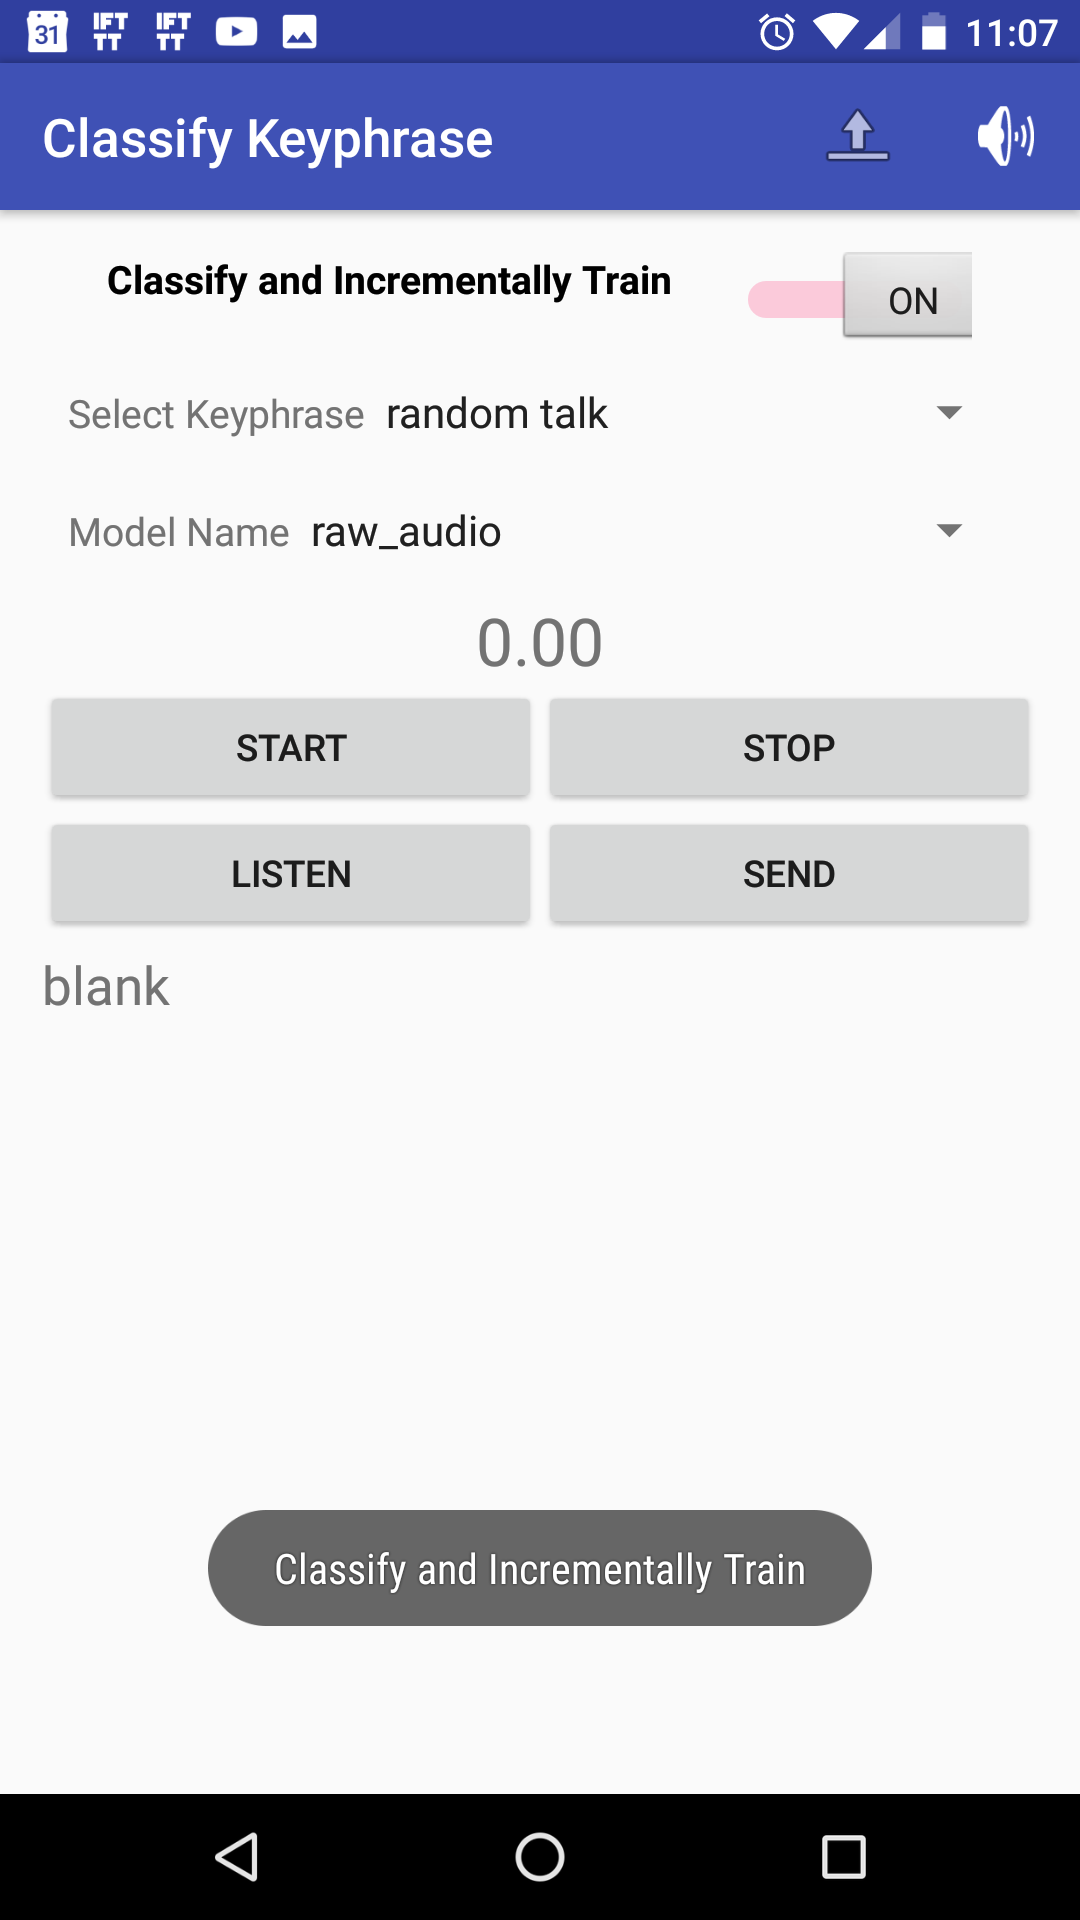
\includegraphics[width=0.5\textwidth]{sound/app_classify_and_train.png}
\caption{Classify and "Fine-Tune" Model}
\end{subfigure}%
\caption{\texttt{dbHound Keyphrase} Android app screenshot for testing the classification models}
\label{fig:dbhound_test}
\end{figure}

For preserving privacy, I propose a two-part solution:
\begin{itemize}
\item A computationally light transformation that removes conversational information from audio but preserves the ability to recognize a desired list of keywords.
\item A computationally light inference technique to spot the keywords from a stream of transformed audio data.
\end{itemize}


